%% 美赛模板:正文部分

\documentclass[12pt]{article}  % 官方要求字号不小于 12 号,此处选择 12 号字体

% 本模板不需要填写年份,以当前电脑时间自动生成
% 请在以下的方括号中填写队伍控制号
\usepackage[2308932]{easymcm}  % 载入 EasyMCM 模板文件.
\usepackage{listings}
\usepackage{xcolor}
\usepackage{booktabs}


% \usepackage{algorithm}
% \usepackage{algorithmicx}
% \usepackage{algpseudocode}
% \usepackage{amsmath}
% \floatname{algorithm}{Algorithm}
% \renewcommand{\algorithmicrequire}{\textbf{Input:}}
% \renewcommand{\algorithmicensure}{\textbf{Output:}}

\usepackage[linesnumbered,ruled,vlined]{algorithm2e}


\usepackage{pythonhighlight}
\usepackage{graphicx}
\usepackage{subfigure}
\usepackage{colortbl}
\usepackage{threeparttable}
\problem{A}  % 请在此处填写题号
% \usepackage{mathptmx}  % 这是 Times 字体,中规中矩 
% 这是 COMAP 官方杂志采用的更好看的 Palatino 字体,可替代以上的 mathptmx 宏包
\usepackage{mathpazo}  


\title{How ?}  % 标题

% 如需要修改题头(默认为 MCM/ICM),请使用以下命令(此处修改为 MCM)
%\renewcommand{\contest}{MCM}
\newenvironment{shrinkeq}[1]
{ \bgroup
	\addtolength\abovedisplayshortskip{#1}
	\addtolength\abovedisplayskip{#1}
	\addtolength\belowdisplayshortskip{#1}
	\addtolength\belowdisplayskip{#1}}
{\egroup\ignorespacesafterend}
% 文档开始
\begin{document}

% 此处填写摘要内容
\begin{abstract}
Finally, we perform a sensitivity analysis of the model and investigate the effect of changes in the variable parameters of the model on the results.

% 美赛论文中需注明关键字。若您一定要使用,
% 请将以下两行的注释号 '%' 去除,以使其生效
 \noindent\textbf{Keywords}: SNA, 

\end{abstract}

\maketitle  % 生成 Summary Sheet
\tableofcontents  % 生成目录


% 正文开始
\section{Introduction}
\vspace{-0.5cm}
\subsection{Problem Background}


\vspace{-0.3cm}
\subsection{Restatement of Problem}
\vspace{-0.3cm}

To bring this grand creature into our world, we need to accomplish the following tasks:

$\bullet$ \textbf{Task1: }Analyzing dragons' features, behavior, habits, diet, and environmental interactions.

\vspace{-0.5cm}
\subsection{Literature Review}
\vspace{-0.3cm}


\subsection{Our Work}
\vspace{-0.3cm}


% \begin{figure}[htbp]
% 	\centering
% 	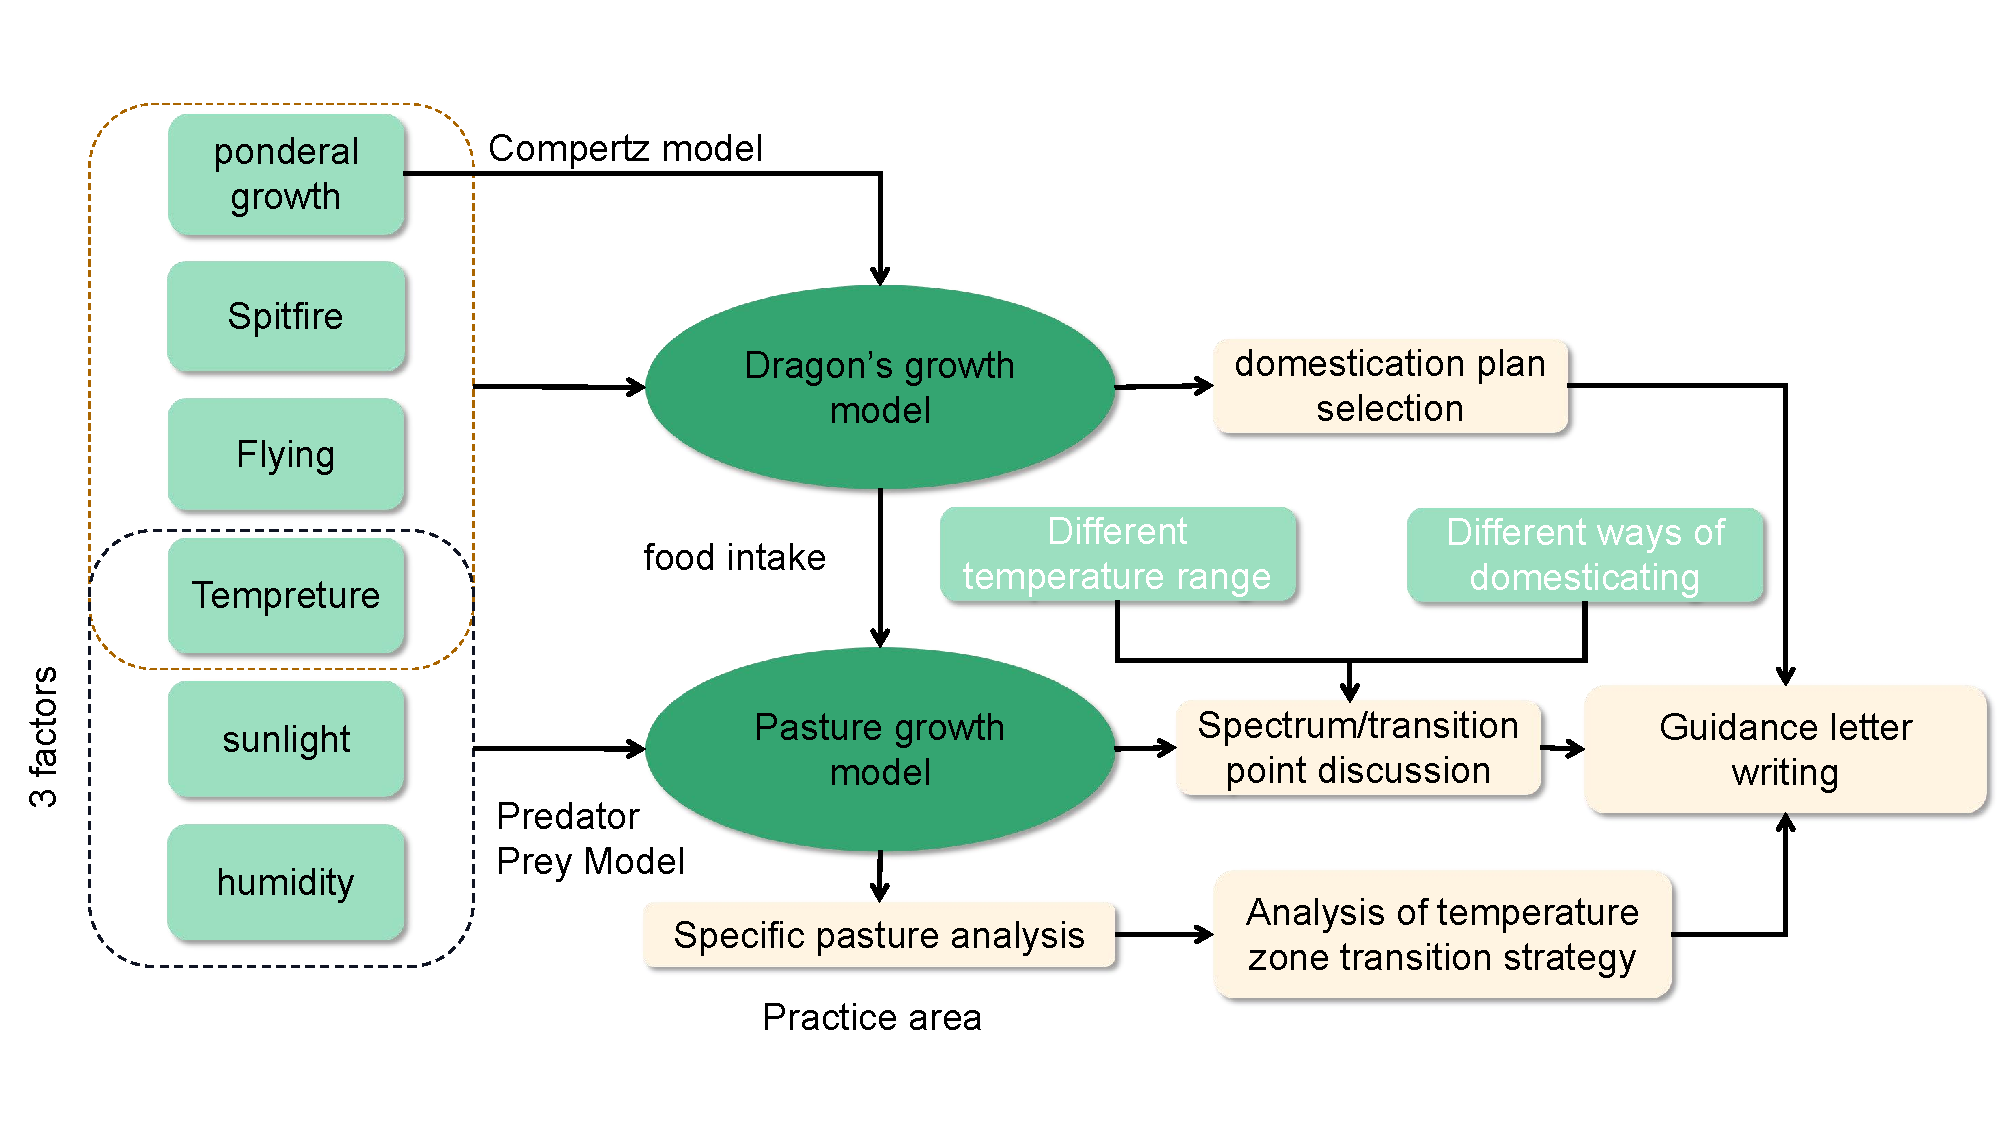
\includegraphics[width=0.85\textwidth]{frame_diagram.pdf}
% 	\caption{Our Work}\label{fig:pic1}
% \end{figure}
% \vspace{-0.3cm}

\newpage

\section{Assumptions and Notations}
\vspace{-0.5cm}
\subsection{Assumptions}
\vspace{-0.3cm}

Through the full analysis of the problem, in order to simplify our model, we make the following reasonable assumptions.
\vspace{-0.5cm}
\begin{itemize}
\item[$\bullet$] \textbf{Assumption1:} Dragons occupy the apex of the food chain.

\vspace{-0.2cm}
\item[$\hookrightarrow $]\textit{\textbf{Justification:}} \textit{Given the formidable offensive and defensive capabilities of dragons, we do not consider any animal to pose a significant threat to their survival.}

\end{itemize}

\subsection{Notations}
\vspace{-0.3cm}
The primary notations used in this paper are listed in Table \eqref{tab:table_one}.
\vspace{-0.4cm}
\begin{table}[!htbp]
	\caption{Parameter Settings}
    \label{tab:table_one}
    \centering
	\begin{tabular}{ccc}
		\toprule[1.5pt]
		\makebox[0.15\textwidth][c]{\textbf{\textit{Symbols}}}	&  \makebox[0.5\textwidth][c]{\textbf{\textit{Description}}}&
        \makebox[0.15\textwidth][c]{\textbf{\textit{Unit}}}	\\
		\toprule[0.75pt]
  
  	$x$ & dynamic Grass production & $t$\\
    	$y$ & The number of sheep & $k$\\

		\bottomrule[1.5pt]
	\end{tabular}
\end{table}
\vspace{-0.6cm}

\newpage

\section{Data preparation}
\vspace{-0.5cm}
\subsection{Data Acquisition \& Pre-processing}
\vspace{-0.3cm}
\subsection{Data Visualization \& Validity Examination}
\vspace{-0.3cm}
\subsection{Clustering Analysis}
\vspace{-0.3cm}

\newpage


\section{Model \uppercase\expandafter{\romannumeral1} : Metabolism of dragon}
\vspace{-0.3cm}





\newpage
\section{Sensitivity Analysis}
\vspace{-0.5cm}

\newpage
\section{Model Evaluation and Further Discussion}
\vspace{-0.5cm}

\subsection{Strengths}
\vspace{-0.3cm}
\begin{itemize}
\item[$\bullet$] \textbf{Accurate Simulation }Our model, which employs the utilization of calories to quantify energy expenditure, effectively concretizes an otherwise abstract concept. Furthermore, in determining energy consumption through activities such as physical exertion and combustion, we employ scientifically rigorous modeling techniques to ensure the utmost precision in our calculations. Additionally, the weather data employed in our model was procured from official sources specific to the location in question, lending a robust practicality to our approach.

\item[$\bullet$] \textbf{Robust Model }As shown in our sensitivity analysis results, our model has strong robustness under both condition 1 and condition 2. Therefore, we believe that our model has good robustness.

\item[$\bullet$] \textbf{Strong Interpretability }In creating our model, we not only maintain a high level of respect and reference to the original works but also combine current world natural science laws to build the model, making the scenario of raising dragons as a magical animal as realistic as possible. For example, by comparing lizards with dragons, we analyze the thermoregulation characteristics of dragons and reference alcohol synthesis combustion to analyze the dragon's fire-breathing process. Through these means, we strive to give the scenario of raising dragons a more realistic sense and thus bring a highly interpretable model.

\item[$\bullet$] \textbf{Universality } Our model, which describes the interactions between dragon cultivation and the surrounding ecosystem, can not only provide insights into dragon-related scenarios, but also has practical applications in evaluating other segments of the ecosystem, such as sheep rearing. Furthermore, it serves as a valuable reference for the conservation of other apex predators of similar nature.
\end{itemize}

 avoid local extremes and thus achieve a global optimal solution

 comprehensiveness and applicability of the evaluation
model.

Data are reliable and accurate.

According to the sensitivity analysis

However, there are weaknesses in the proposed models:

\subsection{Weaknesses}
\vspace{-0.3cm}
\begin{itemize}

\item[$\bullet$] \textbf{Lack Of Real Data }The direct data we have on dragons primarily comes from television show stills and novel source material, however, obtaining data through this method is relatively limited. As a result, we have had to make a fair number of reasonable assumptions and inferences based on scientific facts. This also results in our model deviating from the dragons as imagined by the original authors.

\item[$\bullet$] \textbf{Limited Food Variety }Due to time constraints, we only kept beef and mutton in the dragon's diet, while according to the original work, dragons would also eat many other foods including fish. Therefore, if we consider seafood such as fish and shrimp, we will get different results under specific conditions. For example, in the Arctic, it may be possible to feed dragons by breeding krill, which is certain to make some difference to our current conclusions.



only considered


\end{itemize}
\subsection{Further Improvements}
\vspace{-0.3cm}

In fact, fungal growth is affected by various factors. Quantify predators, PH value,
sunshine and others and We will modify the differential equation to make it more
suitable for common situations. Besides, the analysis and simulation of fungi community can be more accurate if more data can be available. 
\newpage
\section{Article}
\newpage
Article
\newpage
\begin{thebibliography}{99}
	\vspace{-0.5cm}
	\bibitem{1} Zhang Cungang, Li Ming, Lu Demei. \emph{Social Network Analysis: An Important Sociological Research Method} [J]. Gansu Social Sciences, 2004. 
\end{thebibliography}



\newpage
\noindent$\blacktriangleright\ $\textbf{\large{Establishment}}

\textbf{From genre span}: Influence occurs within the same genre and between different genres.
$\bullet$ Applying 

Complex networks are usually called scale-free networks\cite{1},as is shown in the Table\eqref{tab:best}.The cosine similarity between the eigenvectors of music A and music B $S_{cos}(\mathbf{A},\mathbf{B})$ is defined by the following equation\eqref{eq:cos}


The work we have done in this problem is mainly shown in the following Figure\eqref{fig:work1}.
\vspace{-0.3cm}
\begin{figure}[htbp]
	\centering
	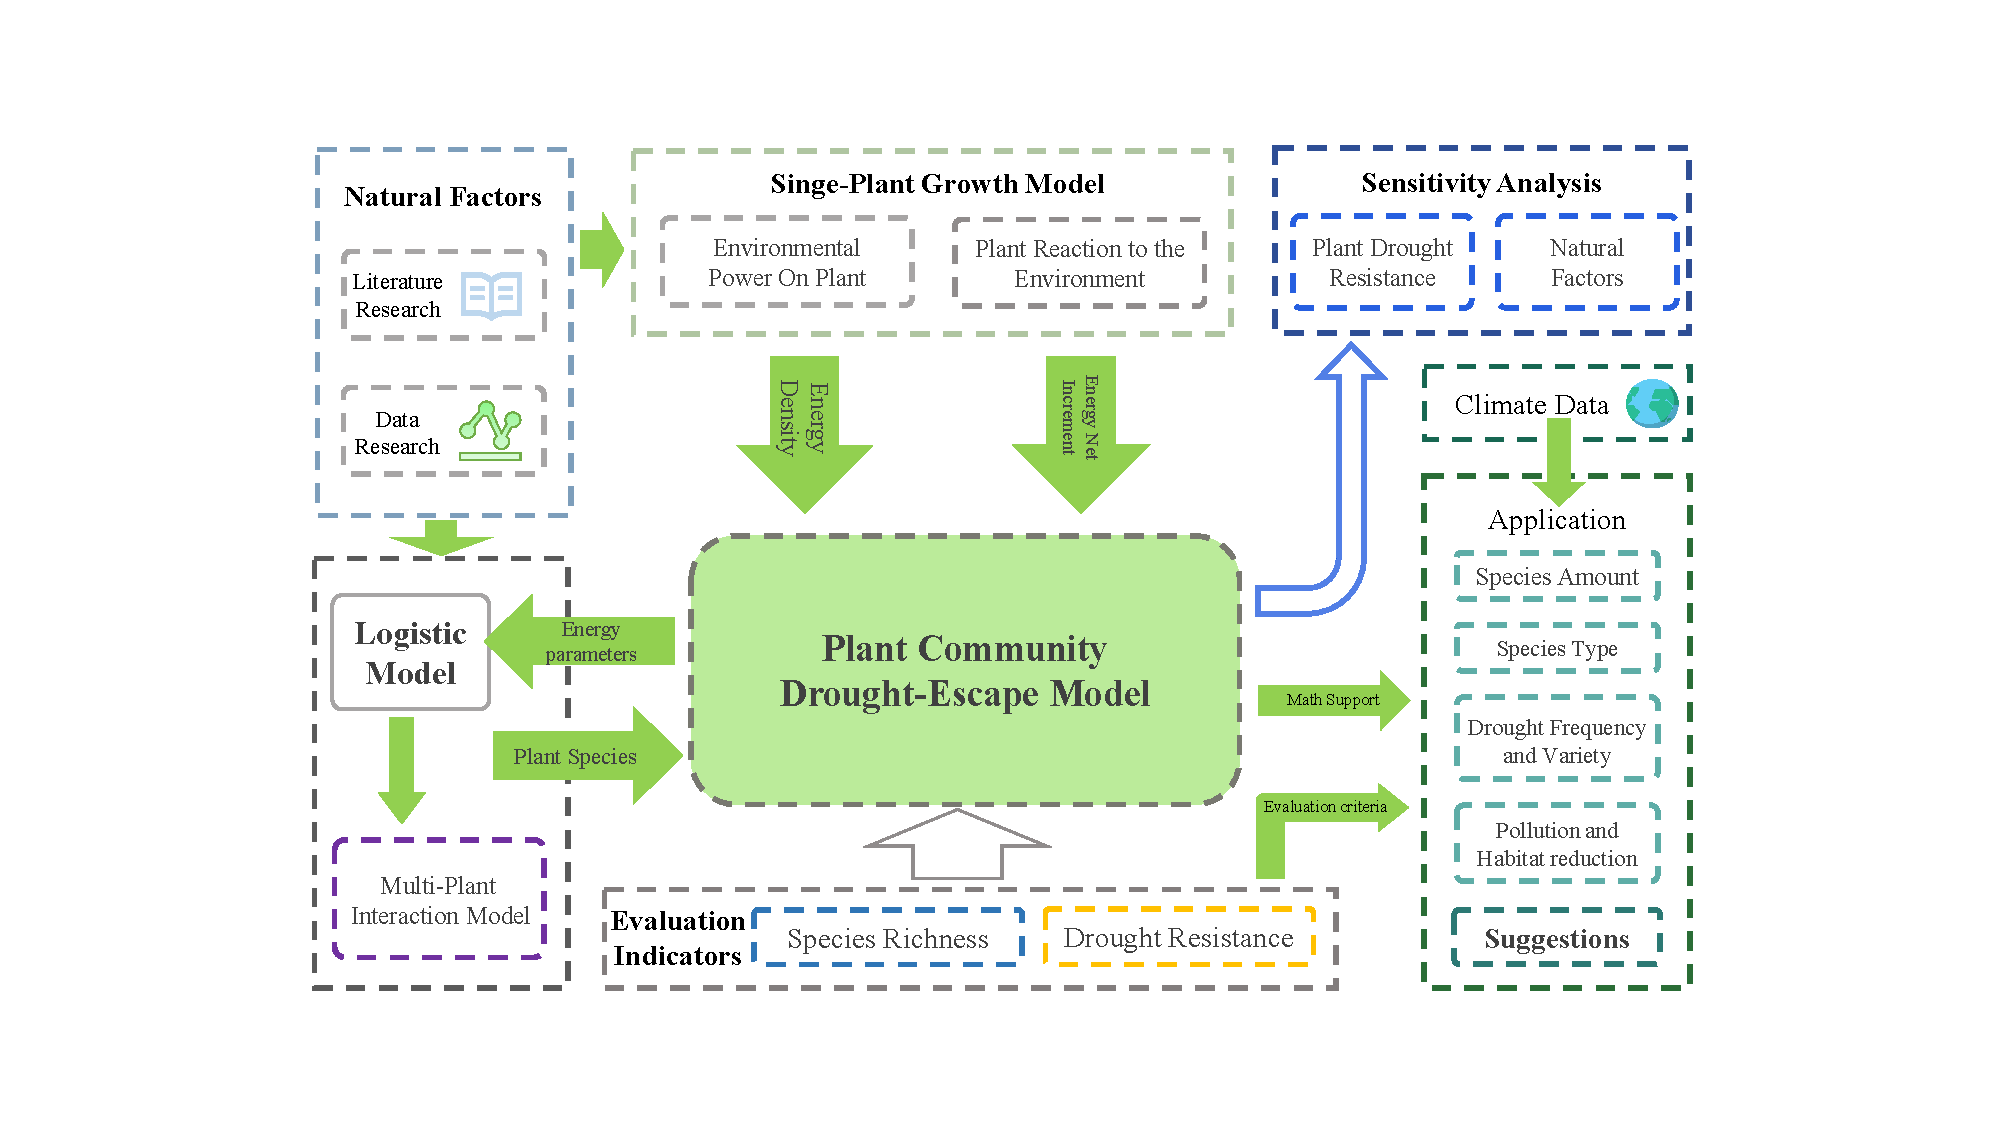
\includegraphics[width=0.5\textwidth]{work.pdf}
	\caption{Our Work}\label{fig:work1}
\end{figure}
\vspace{-0.3cm}

\begin{figure}[htbp]
	\centering
	\begin{minipage}[t]{0.45\textwidth}
		\centering
		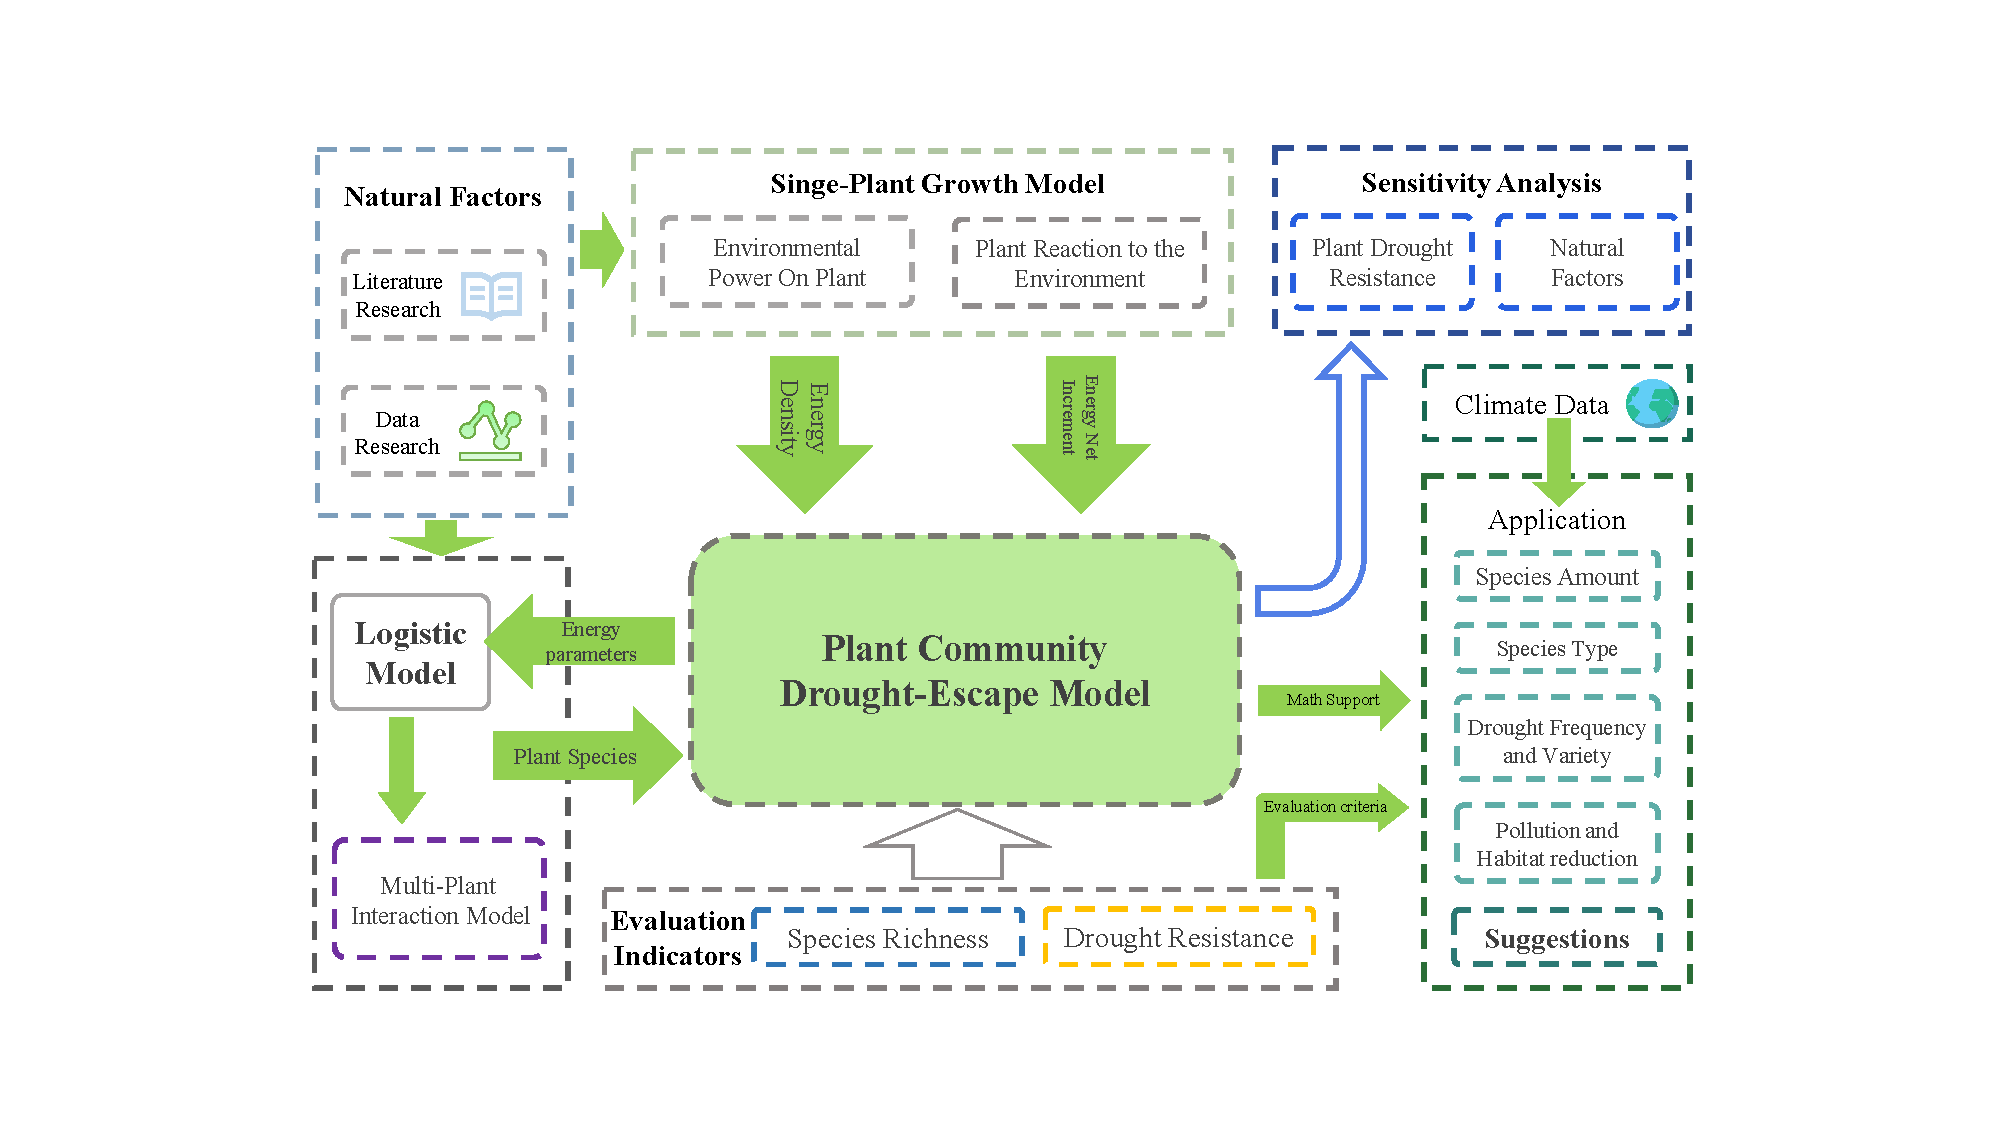
\includegraphics[width=1\textwidth]{work.pdf}
		\caption{Global Similarity}\label{fig:quanju}
	\end{minipage}
	\begin{minipage}[t]{0.45\textwidth}
		\centering
		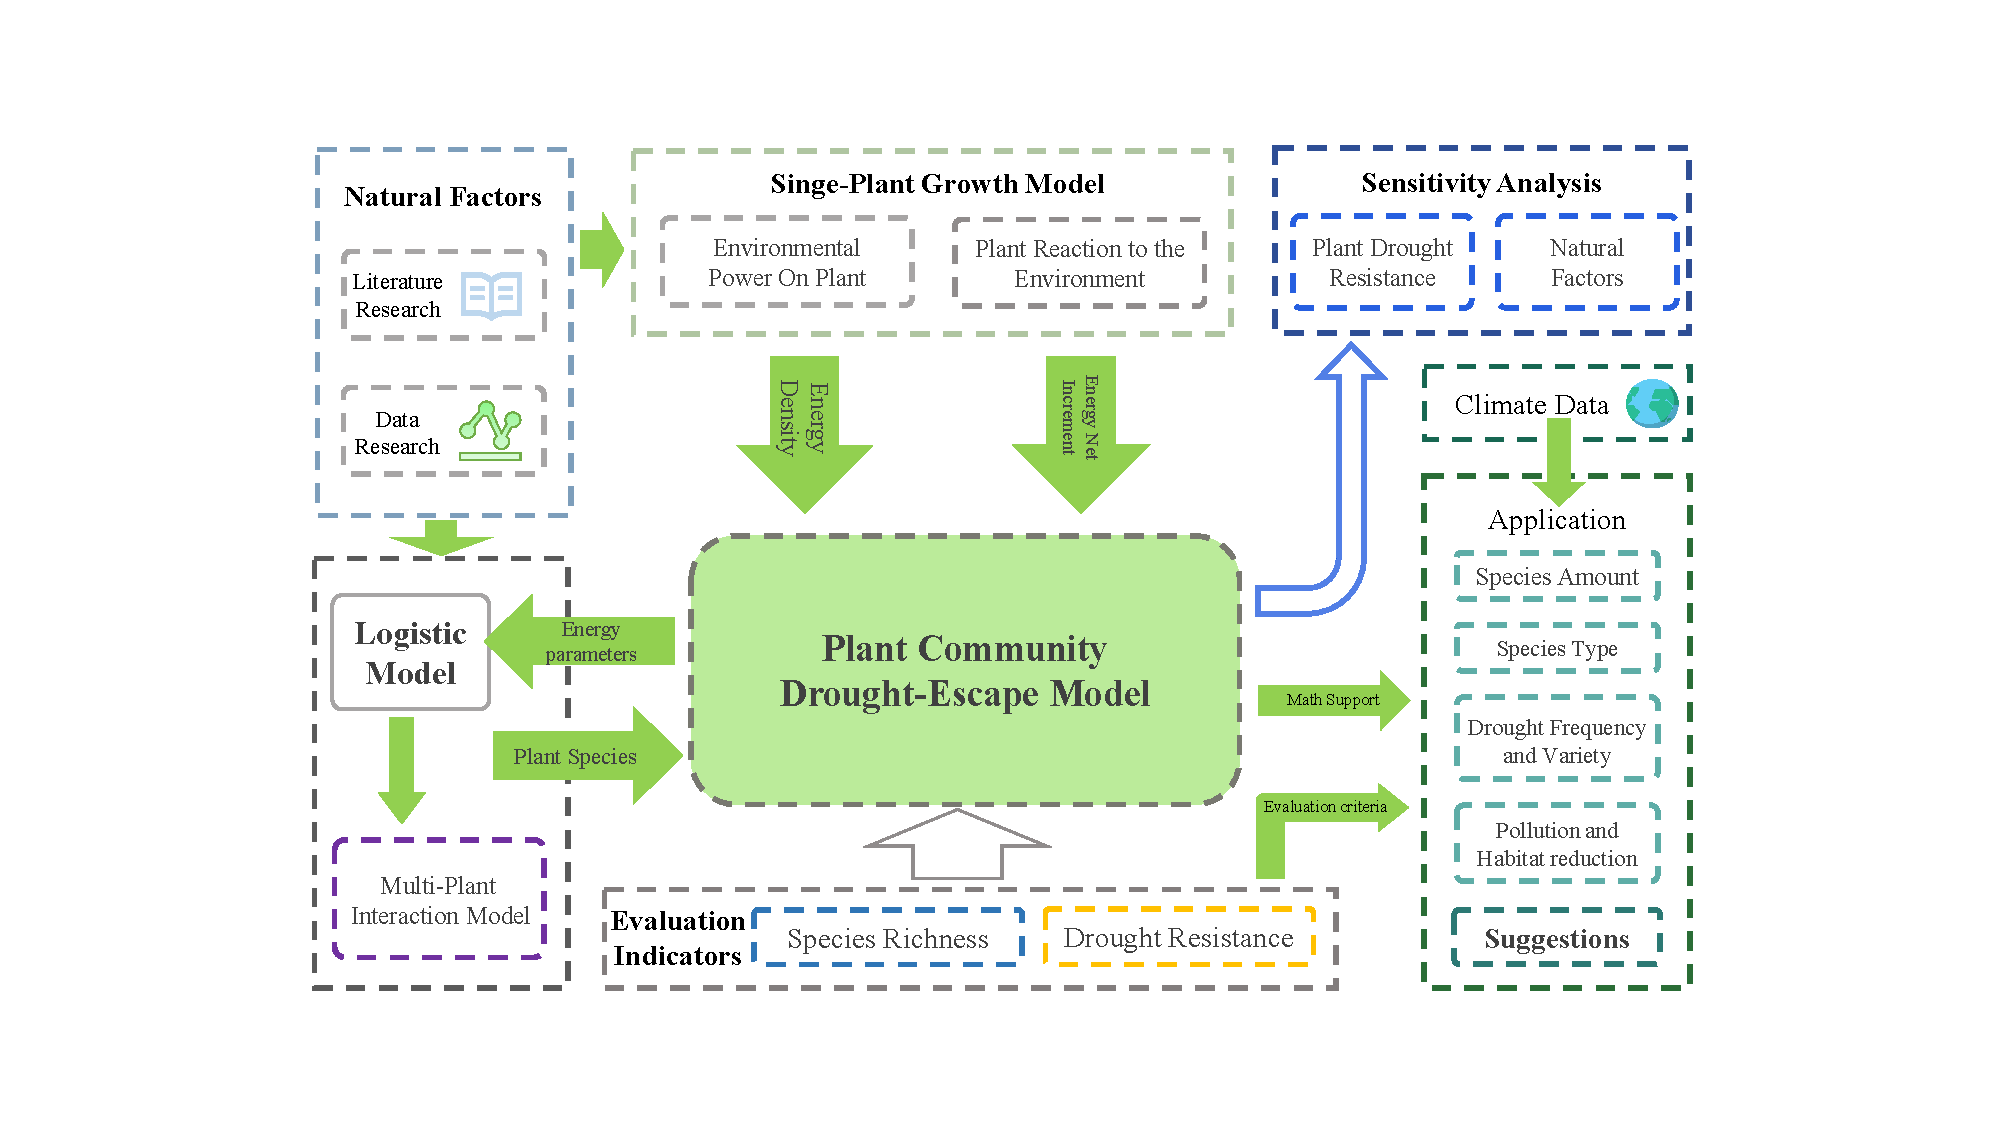
\includegraphics[width=0.98\textwidth]{work.pdf}
		\caption{Multi--Similarity}\label{fig:jubu}
	\end{minipage}
\end{figure}


\begin{figure}[htbp]
\begin{minipage}[b]{0.5\linewidth}
The food system can be defined as a complete set of people, institutions, activities, processes and infrastructure involved in the production and consumption of food by a certain population. Specifically, it includes planting, harvesting, processing, packaging, transportation, and marketing activities related to the food system, and any inputs required at each step along the chain of activities, such as land, agricultural chemicals, labor, water,machinery, capital) and out
put.      
\end{minipage}
\hfill
\begin{minipage}[b]{0.45\linewidth}
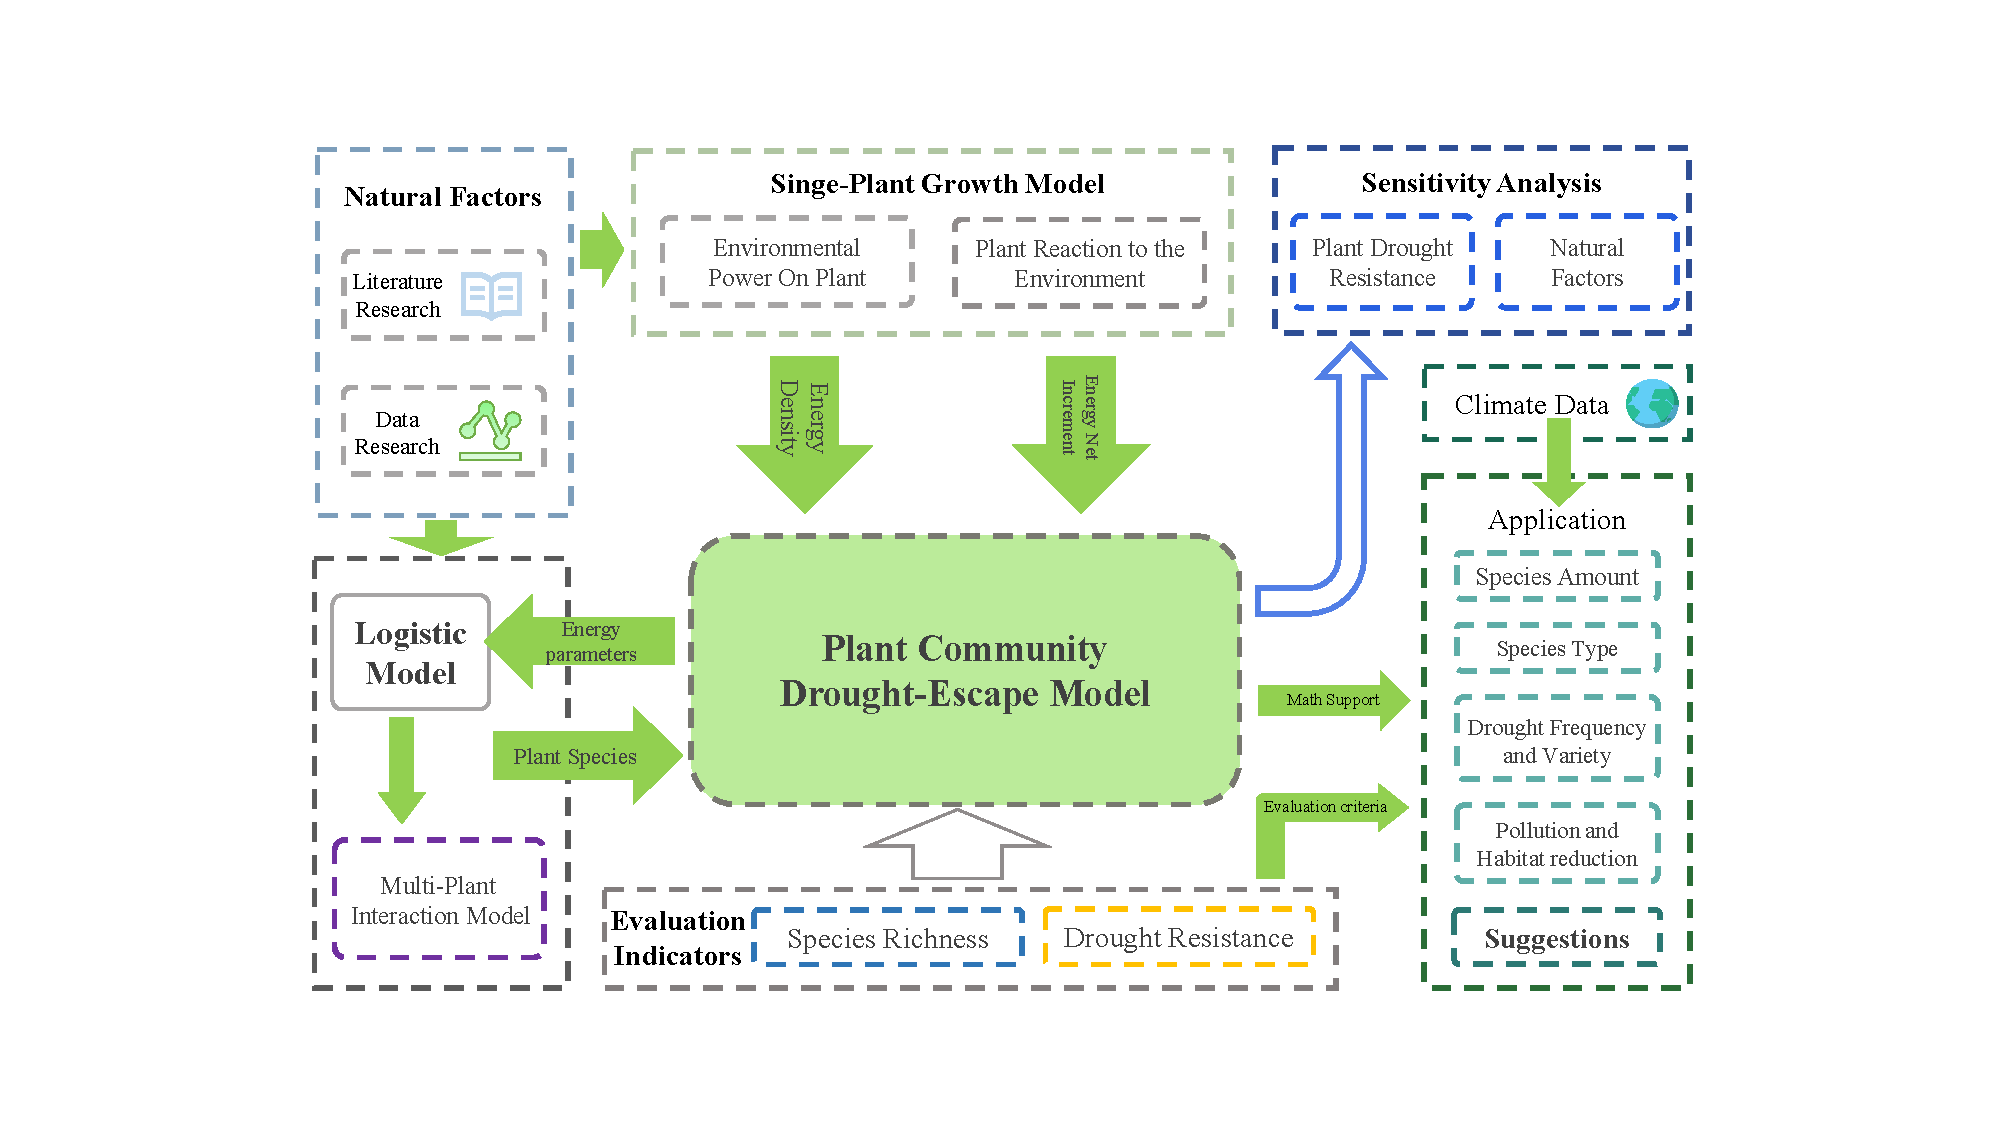
\includegraphics[height=8\baselineskip]{work.pdf}
\caption{Our Work}
\end{minipage}
\end{figure}

\IncMargin{1em}
\begin{algorithm} 
\SetKwData{Left}{left}
\SetKwData{This}{this}
\SetKwData{Up}{up} 
\SetKwFunction{Union}{Union}
\SetKwFunction{FindCompress}{FindCompress} \SetKwInOut{Input}{input}
\SetKwInOut{Output}{output}
	
	\Input{A bitmap $Im$ of size $w\times l$} 
	\Output{A partition of the bitmap}
	\BlankLine 
	 
	 \emph{special treatment of the first line}\; 
	 \For{$i\leftarrow 2$ \KwTo $l$}{ 
	 	\emph{special treatment of the first element of line $i$}\; 
	 	\For{$j\leftarrow 2$ \KwTo $w$}{\label{forins} \Left$\leftarrow$\FindCompress{$Im[i,j-1]$}\; 
	 	\Up$\leftarrow$ \FindCompress{$Im[i-1,]$}\; 
	 	\This$\leftarrow$ \FindCompress{$Im[i,j]$}\; 
	 	\If(\tcp*[h]{O(\Left,\This)==1})
	 		{\Left compatible with \This}{\label{lt} 
	 			\lIf{\Left $<$ \This}{\Union{\Left,\This}}
	 			 \lElse{\Union{\This,\Left}} } }
 		 \lForEach{element $e$ of the line $i$}{\FindCompress{p}} 
 	 } 
        \caption{disjoint decomposition}
        \label{algo_disjdecomp} 
        \end{algorithm}
 \DecMargin{1em} 


% \subsubsection{Parameter Rectification}
%     \begin{algorithm}
% 	\caption{Draw the Power Curve}
% 	\begin{algorithmic}[1] %每行显示行号
% 		\Require $k_f$,$k_r$,$k_{\rm in}$,$k_{\rm out}$,$P_{\rm max0}(J)$,$E_0(J)$:Parameters for the athlete
% 		\Ensure the Power Curve of the athlete
% 		\State $t_{\rm list}=\textbf{[]}$
% 		\State $P_{\rm rider\_list}=\textbf{[]}$		
% 		\For {$P_{\rm rider} = 100; P_{\rm rider}<1500; P_{\rm rider}++$}
% 		\State $E=E0$
% 			\For {$i = 100; i<800; i++$}
% 			\State $update \ the \ value \ of \ P_{\rm max}$
% 			\State $update \ the \ value \ of \ E$		
% 				\If $P_{\rm rider}>P_{\rm max} or E<0$
% 				\State $t=i$
% 				\State $break$
% 				\EndIf
% 			\EndFor
% 		\State $t_{\rm list}.append(t)$
% 		\State $P_{\rm rider\_list}.append(P_{\rm rider})$		
% 		\EndFor
% 		\State $plot(t_{\rm list}, P_{\rm rider_list})$
% 	\end{algorithmic}
% \end{algorithm}


% Table generated by Excel2LaTeX from sheet 'Sheet2'
\begin{table}[htbp]
  \centering
  \caption{Add caption}
    \begin{tabular}{c|c|c|c|c}
    \hline
    \hline
    \rowcolor[rgb]{ 1,  .902,  .6} A     & \multicolumn{2}{c|}{\cellcolor[rgb]{ .886,  .937,  .855} B} & \multicolumn{2}{c}{\cellcolor[rgb]{ 1,  .4,  0} C} \\
    \hline
    \rowcolor[rgb]{ 1,  .902,  .6} A     & \cellcolor[rgb]{ .886,  .937,  .855} B & \cellcolor[rgb]{ .886,  .937,  .855} B & \cellcolor[rgb]{ 1,  .4,  0} C & \cellcolor[rgb]{ 1,  .4,  0} C \\
    \hline
    \rowcolor[rgb]{ 1,  .902,  .6} A     & \cellcolor[rgb]{ .886,  .937,  .855} B & \cellcolor[rgb]{ .886,  .937,  .855} B & \cellcolor[rgb]{ 1,  .4,  0} C & \cellcolor[rgb]{ 1,  .4,  0} C \\
    \hline
    \hline
    \end{tabular}%
  \label{tab:best}%
\end{table}%

\begin{shrinkeq}{-1ex}
	\begin{equation}\label{eq:glo}
	S_{global}(\mathbf{A},\mathbf{B})=S_E(\mathbf{A},\mathbf{B})+S_{cos}(\mathbf{A},\mathbf{B})
	\end{equation}
\end{shrinkeq}

\begin{shrinkeq}{-1.5ex}
	\begin{equation}
	distance_{AB}=\sqrt{\sum\limits_{i=1}^{n}(A_i-B_i)^2}
	\end{equation}
\end{shrinkeq}

\begin{shrinkeq}{-1.5ex}
	\begin{equation}\label{eq:cos}
	S_{cos}(\mathbf{A},\mathbf{B})=1+\frac{cos\theta}{2}=1+\frac{\mathbf{A}\cdot\mathbf{B}}{2\cdot||\mathbf{A}||\cdot||\mathbf{B}||}=1+\frac{1}{2}\cdot\frac{\sum\limits_{i=1}^{n}A_i\cdot B_i}{\sqrt{\sum\limits_{i=1}^{n}(A_i^2)}+\sqrt{\sum\limits_{i=1}^{n}(B_i^2)}}
	\end{equation}
\end{shrinkeq}

\begin{shrinkeq}{-1.5ex}
	\begin{equation}\label{eq:control}
		\begin{cases}
		|v_3^{(k)}-v_2^{(k)}|<0.03\\
		|v_2^{(k)}-v_1^{(k)}|<0.03\\
		|v_4^{(k)}-v_3^{(k)}|>0.1\\
		|(v_5^{(k)}-v_4^{(k)})-(v_4^{(k)}-v_3^{(k)})|<0.02\ or\ |v_5^{(k)}-v_4^{(k)}|<0.03\\
		|(v_6^{(k)}-v_5^{(k)})-(v_5^{(k)}-v_4^{(k)})|<0.02\ or\ |v_6^{(k)}-v_5^{(k)}|<0.03
		\end{cases}
	\end{equation}
\end{shrinkeq}



% 以下为信件/备忘录部分,不需要可自行去掉
% 如有需要可将整个 letter 环境移动到文章开头或中间
% 请在后一个花括号内填写信件(Letter)或备忘录(Memorandum)标题
\begin{letter}{MEMO\centering}
	\begin{flushleft}  % 左对齐环境,无首行缩进
		\textbf{To:} \textbf{Experts in The ICM Society}\\
		\textbf{From:} \textbf{Team 2300000}\\
		\textbf{Date:} \textbf{February 19th, 2023}\\
		\textbf{Subject:} \textbf{How ?}
	\end{flushleft}

\noindent Dear experts in the ICM Society:

 We are honored to inform you our achievement after  performing data analysis and establishing the music influence and similarity evaluation model. 

\end{letter}



% \begin{subappendices}  % 附录环境
	
% \section{Appendix A: Further on }
% To clarify the importance of using \LaTeX\ in MCM or ICM, several points need to be covered, which are \ldots

% To be more specific, \ldots

% All in all, \ldots

% Anyway, nobody \textbf{really} needs such appendix \ldots

% \section{Appendix B: Program Codes}
% Here are the program codes we used in our research.

% % Python 代码示例
% \begin{lstlisting}[language=Python, name={test.py}]
% # Python code example
% for i in range(10):
%     print('Hello, world!')
% \end{lstlisting}


% % MATLAB 代码示例
% \begin{lstlisting}[language=MATLAB, name={test.m}]
% % MATLAB code example
% for i = 1:10
%     disp("hello, world!");
% end
% \end{lstlisting}

% \end{subappendices}

\end{document}  % 结束